\documentclass{article}
\usepackage{graphicx}
\usepackage{amssymb}
\usepackage{amsmath}
\usepackage{multicol}

\usepackage{todonotes}
\usepackage{float}
\usepackage{booktabs}
\usepackage{subfig}
\usepackage{placeins}
\usepackage{url}
\usepackage{lineno}

\title{TREMA-UNH at TREC 2018: Complex Answer Retrieval and News Track}

\author{Sumanta Kashyapi, Shubham Chatterjee, Jordan Ramsdell, Laura Dietz \\
\texttt{\{sk1105, sc1242, jsc57\}@wildcats.unh.edu, dietz@cs.unh.edu}\\
TREMA lab, University of New Hampshire, U.S.A}
\date{} 

\begin{document}

\maketitle 
%% Title, authors and addresses

\begin{abstract}
This notebook describes the submission of team TREMA-UNH to the TREC Complex Answer Retrieval track and the TREC News track in 2018. Our methods focus on passage retrieval, entity-aware passage retrieval, and entity retrieval.
\end{abstract}

%% main text
\section{Introduction}
\label{S:1}

Users expectations of search engines continue grow with advancements of search engines and retrieval models. We explore ``search engines of the future'' that not only rank documents according to relevance, but also present all relevant information in a compact manner from which users are able to synthesize knowledge easily.  To accomplish this task, we train retrieval models to have a better understanding relevance for natural language. 

The Complex Answer Retrieval (CAR)\cite{trecdata21} track at the Text Retrieval Conference (TREC)\footnote{\url{https://trec.nist.gov}} aims to address this scenario. Current retrieval systems provide good solutions towards passage retrieval for simple fact and entity-centric information needs.
In contrast, CAR is about answering more complex information needs with longer answers.
The formal task statement includes the two following tasks:

\noindent \textbf{CAR Passage Task:} Given an article stub $Q$, retrieve for each of its sections $H_i$, a ranking of relevant passages $P$. The passage $P$ is taken from a provided paragraph corpus. %that is the name of the corpus!

\noindent \textbf{CAR Entity Task:} Given an article stub $Q$, retrieve for each of its sections $H_i$, a ranking of relevant entities $E$. The entity $E$ is taken from a provided Wikipedia corpus. Additionally for each entity $E$, a support passage from the passage corpus is to be identified that explains why the entity is relevant for the heading $H_i$ on the stub.
\medskip

\noindent We further participate in the NEWS track entity ranking task. 

\noindent \textbf{NEWS Entity Task:} Given a news article with title and content that is annotated with entity links to a set of entities  $\mathcal{E}=\{E1, E2, ... En\}$, the task is to rank the the given entities by importance for the article (i.e., saliency). 

\medskip 

\section{Overarching Approach}
\label{sec:overarching}
 For each page, we use the section headings from the page's outline as queries. The headings are usually very short. Hence, using retrieval models without query expansion (such as BM25) may not yield good results since headings have potentially little textual overlap with their passages. To alleviate this problem, we experiment with various entity- and word-based query expansion methods. We observe the performance of each of the methods individually. However, since any single unsupervised method may not provide best performance on its own, we also experiment with machine-learned combinations of methods using learning-to-rank.\footnote{\url{http://lemurproject.org/ranklib.php}} 

A knowledge graph (KG) is used to enhance a retrieval models's results with information gathered from a variety of sources. The KG provides access to knowledge about entities and is derived from external sources such as Wikipedia. Here we use a Wikipedia dump\footnote{\texttt{unprocessedAllButBenchmark.v2.1.tar.xz}, Wikipedia dump from December 2016} provided by the TREC CAR organizers that does not include pages from test queries. Such knowledge graphs hold a wealth of information which can be leveraged to solve information retrieval problems. 

In Section \ref{sec:para} we first describe which unsupervised retrieval and expansion models were used for the passage task, and in Section \ref{sec:entity} for the entity task.  

%This was already said above.
%The section headings and paragraphs in the TREC-CAR dataset are not generated from the same model. Section headings are constructed in such a way that they best capture the prevalent ideas expressed in the paragraphs under them. Conversely, paragraphs could be seen as elaboration of the the section heading. Hence, for the passage retrieval task, there is little chance of success if we try to directly map section headings to paragraph texts. Hence, we try to estimate the language model over top-k TF-IDF words of the feedback run and use it to map paragraphs to section headings.


%\section{Related Work and Background}
%\label{S:2}
\section{Low-level Retrieval Features}
\label{sec:low-level}

Each of our approaches are based on a variety of unsupervised retrieval models and document indexes that we describe in the following.

\paragraph{Indexes:}

We create the following indexes for use with our retrieval methods. 
\begin{itemize}
    \item A paragraph index out of the text in passages of the \texttt{paragraphCorpus}.
    \item A page index out of all visible text on Wikipedia pages in \texttt{allButBenchmark}. 
    \item An entity index out of the first paragraph, anchor text, and category info of Wikipedia in \texttt{allButBenchmark}.
%    \item An ecm-paragraph index out of text in paragraphs in Wikipedia pages in \texttt{allButBenchmark}.
\end{itemize}



\paragraph{Query models:}
Given a stub with page title $T$ and a tree-shaped outline of headings $H1$, $H1.1$, $H1.2$, $H1.2.1$, $H2$,... there are different ways to derive queries for retrieval with BM25, QL, etc for text of a particular heading, such as $H1.2$. The simplest approach is what we call \textit{section path queries}, which concatenates the page title, $T$, with all parent headings (in this example $H1$), along with the heading itself ($H1.2$), to derive the query. However, more options are possible such, as as:

\begin{itemize}
    \item Section Path: Concatenation of page title, parent headings, and heading (Example: $T, H1, H1.2$).
    \item Title: only the page title ($T$)
    \item Leaf: only the heading itself ($H1.2$)
    \item Internal: concatenation of the parent heading(s) ($H1$)
    \item All: concatenation of page title and all headings in the stub \\ ( $T, H1, H1.1, H1.2, H1.2.1, H2, \dots$ )
    \item Subtree: concatenation of all headings in the subtree rooted by the heading ($H1.2, H1.2.1$)
\end{itemize}

The section path model is very popular among the TREC CAR participants and usually works best as a standalone method. However, it has been argued that learning a weighted combination between title, internal, and leaf query models could give potentially even better performance \cite{macavaney2018overcoming}.


\paragraph{Retrieval and expansion models:}

Given a query model to transform the stub into a keyword query and an index, and we  use different retrieval models to obtain low-level rankings (which we will combine with different learning to rank methods in the following). In particular we use as retrieval models:

\begin{itemize}
    \item BM25, as implemented in Lucene (using default parameters).
    \item Query likelihood with Dirichlet smoothing, as implemented in Lucene.
\end{itemize}

We use as expansion models    
\begin{itemize}
    \item None: No expansion. Just uses the initial ranking.
    \item RM3: RM Relevance model expansion \cite{lavrenko2017relevance} using 20 top paragraphs/pages to expand with 20 terms. This is an RM1-style ranking that is intended to be combined with the basic ranking model (to yield RM3).
    \item ECM: A variant of RM3 representing a document as a bag-of-entity-link-targets. Uses top 100 paragraphs/pages.
    \item ECM-psg: Like ECM expansion but expands the keyword query with top 100 expansion entities.
\end{itemize}

Ecm uses the entity context model in a non-standard way, where the whole page is used instead of short passages: After retrieving a feedback run of paragraphs or Wikipedia pages with BM25, each page is represented as bag-of-entity-link-targets. Using the relevance model \cite{lavrenko2017relevance}, we compute the distribution over expansion entities $P(E|Q)$. We discuss two variants, in \textbf{ecm-passage} we expand the query with these entities to retrieve a new ranking. In \textbf{ecm} we use the distribution directly to produce a ranking of entities.

$$ score(E|Q)= \sum_{D\in \text{ranking}} p(D|Q) p(E|D)$$

The name ecm is in attribution to the entity context model \cite{dalton2014entity}, which uses passages with contained entity mentions for new expansion models. Where Dalton et al.\ \cite{dalton2014entity} uses passages surrounding entity links in a feedback run, the ecm-paragraph index allows us to directly retrieve relevant passages with entity-centric information.


We provide all low-level runs for benchmarkY1train, benchmarkY1test and benchmarkY2test online.\footnote{Available at \url{http://trec-car.cs.unh.edu/runs/TREMA-UNH}} 


\subsection{Low-level Paragraph Retrieval Features}\label{sec:para}

We  use the following pararaph ranking and expansion models to derive features for  learning-to-rank for the passage task (decribed in the following sections).
\begin{itemize}
    \item sectionPath-bm25-none: Using section path queries, BM25 retrieval model (no expansion) 
    \item sectionPath-ql-none: Using section path queries, Query likelihood retrieval model (no expansion)
    \item sectionPath-bm25-rm: Using section path queries, BM25-based RM3
    \item sectionPath-ql-rm: Using section path queries, query likelihood-based RM3
\end{itemize}

The results of low-level retrieval methods are presented in Table \ref{tab:para}.

\begin{table}[tb]
\centering
\begin{tabular}{l l l l}
\hline
\textbf{Feature} & \textbf{MAP} & \textbf{Rprec} & \textbf{recip\_rank}\\
\hline
sectionPath-bm25-none & 0.1291 & 0.1031 & 0.2006 \\
sectionPath-ql-none & 0.1232 & 0.0939 & 0.1888 \\
sectionPath-bm25-rm & 0.1038 & 0.0767 & 0.1657 \\
sectionPath-ql-rm & 0.0744 & 0.0493 & 0.1180 \\
\hline
\end{tabular}
\caption{Paragraph feature results, Y1 Train tree qrels}\label{tab:para}
\end{table}

\subsection{Low-level Entity Retrieval Features}
\label{sec:entity}


We  use the following ranking and expansion models to derive features for  learning-to-rank for the entity task (decribed in the following sections).


\begin{itemize}
\item sectionPath-bm25-ecm: Using section path queries, BM25 ranking with ECM ranking based on BM25 page retrieval.
\item sectionPath-ql-ecm: Same as above, but based on Query likelihood.
\item all-bm25-ecm: Constructing a query from title and all headings on the outline,  ECM ranking based on BM25 page.
\item all-ql-ecm: Same as above, but based on Query likelihood.

%   \item query-level: section path, all
%    \item retrieval-model: BM25, Query Likelihood
%    \item expansion-model: Entity Context Model
    \end{itemize}

These were then combined using  learning-to-rank and a combined ranking was obtained. 
This model is trained on benchmarkY1-train, using the tree-level ground truth for the passage task.    

\section{UNH-p-l2r}

Interpreting the set of rank scores (using Section \ref{sec:para}) for a particular paragraph as features, we learn how to optimally combine these features into a weighted combination. We train the model using the coordinate ascent algorithm of RankLib's learning to rank implementation, optimized for mean average precision. 

We train combinations of:
\begin{itemize}
    \item sectionPath-bm25-none: BM25 retrieval model
    \item sectionPath-ql-none: Query likelihood retrieval model (no expansion)
    \item sectionPath-bm25-rm: BM25-based relevance feedback
    \item sectionPath-ql-rm: Query likelihood-based relevance feedback
\end{itemize}

\section{UNH-e-l2r}

Using Lucene indexes for %aspect,
entity, page and paragraph (as described in Section \ref{sec:low-level}). We create features for each index by combining query-level, retrieval-model, and expansion-model methods as follows:

We train combinations of (across all choices of entity, page and paragraph indexes):
\begin{itemize}
    \item sectionPath-bm25-ecm: Section-path BM25 retrieval model with ecm entity ranking
    \item sectionPath-ql-ecm: Same as above but with Query likelihood instead of BM25
    \item all-bm25-ecm: Query from title and all headings using BM25 retrieval model with ecm entity ranking
    \item all-ql-ecm: Same as above but with Query likelihood instead of BM25
\end{itemize}


%Different indexes for retrieving entities and paragraphs are built from allButBenchmark and paragraphCorpus to obtain 10 rankings over Wikipedia pages or paragraphs. Using the entity context model, we build entity relevance models (rankings over entity ids) from the pages/paragraphs, which are used as a ranking of entities. The particular run files are created by using a section path query to retrieve from these indices with BM25 and query likelihood. Additionally, paragraphs are retrieved by building a query from all headings of the topic page.

These were then combined using  learning-to-rank and a combined ranking was obtained. 
This model is trained on benchmarkY1-train, using the tree-level ground truth for the entity task.

The rankings were annotated with the highest ranked paragraph from an additional paragraph ranking as described below.


\section{UNH-p-SDM}\label{sec:sdm}

We use Lucene to index the TREC CAR 2017 paragraph corpus after stemming and removing stopwords.
The UNH-p-SDM method is inspired by the Sequential Dependence model \cite{metzler2005markov} in that it combines unigrams, bigrams, and windowed-bigrams. However, where the original approach by Metzler et al.\ used language models (such as query likelihood) as features, here we use BM25 as a basis for scoring the relevance of documents given a query. We do so by indexing the unigrams, bigrams, and unordered windowed-bigrams (with a window size of eight words) as document fields using Lucene. We tokenize and stem documents using Lucene's English analyzer. We then consider three features that score document relevance with respect to these fields:
 
 \begin{itemize}
     \item Unigram: Unigrams in the query are used to retrieve and score passages via their unigram fields.
     \item Bigram: Bigrams in the query are used to retrieve and score passages via their bigram fields with BM25/QL.
     \item Windowed-bigram: Unordered windowed bigrams in the query are used to retrieve and score passages via their windowed bigram fields. 
 \end{itemize}
 

We train a weighted combination of these three scores that best predicts the relevance of a passage.  We do so by using RankLib with coordinate ascent, optimized for best MAP performance. 


\section{Joint Entity-Passage Methods}\label{sec:joint}


%\subsection{Transforming Features}\label{sec:joint}
In this paper, we explore features that can be used to jointly score entities and passages. We do so using the following approaches.

\textbf{Passage retrieval using entity features.} Let $f_e$ be an entity relevance feature.
For each passage, $p$, let $E$ be the set of entities contained in $p$.
Then a feature that scores the relevance of $p$ given the relevance entities can be represented as $f_p(p) = \sum_{e \in E}{f_e(e)}$. 
We are free to combine this feature with other passage features to rank retrieved passages according to relevance.

\textbf{Entity retrieval using passage features.} Let $f_p$ be a passage relevance feature.
For each entity, $e$, let $P$ be the set of passages (retrieved with UNH-p-SDM) that contain at least one instance of $e$.
We may sum over the scores of passages that contain $e$ to produce a score for $e$: $f_e(e) = \sum_{p \in P}{f_p(p)}$.

\subsection{Description of Passage Features}\label{sec:jointpassage}
We consider the following passage features for use in our joint entity-passage methods:

\textbf{UNH-p-SDM.} We directly use the scores of passages obtained by the UNH-p-SDM (see section~\ref{sec:sdm})) passage retrieval method as a passage feature. 

\textbf{SDM.} Passages are scored using a standard SDM model under query likelihood, in the spirit of Metzler et al.\ \cite{metzler2005markov}.

We convert these passage features into into entity features as described above.


\subsection{Description of Entity Features}\label{sec:jointentity}
We consider the following entity features for use in our joint entity-passage methods:


\textbf{Entity Link Frequency. } We score an entity with respect to the relative frequency at which it was linked to by passages in a candidate set of passage. We do so by summing over the total number of times an entity was linked by candidate passages, and then normalizing by the total number of entity links among all candidate passages. %This feature is used either directly as an entity feature, or is transformed to a passage feature by summing over the relative entity frequencies of entities contained within a passage. 


\textbf{Fielded Queries.} Because our entity index represents a collection of Wikipedia pages, we can consider page attributes as document fields. We store the following page attributes as unigrams in document fields: (enwiki) categories, inlinks, outlinks, section headers, page name disambiguations, and page name redirects. We score the relevance of entities with respect to the query by using the standard BM25 model.  This feature can also be transformed into a passage feature.


\textbf{Global Entity Context.} Whenever a passage links to an entity in Wikipedia, we create a pseudo-document that contains the unigrams, bigrams, and windowed bigrams derived from that passage.  We consider the collection of all such pseudo-documents belonging to an entity as that entity's ``context'' in which it is mentioned. This differs from query-specific context models  \cite{dalton2014entity}, in that we use one global entity context model derived from the corpus. For each query, we construct a unigram, bigram, and windowed bigram query that is used to retrieve pseudo-documents from the global entity context index. 

Pseudo-documents are scored with respect to the standard BM25 model.
Each pseudo-document represents a particular context in which an entity is mentioned in a passage, and we let an entity's score be equal to the highest scored context in which it was mentioned. We obtain one such score for each of the retrieval methods (unigrams, bigrams, and windowed bigrams). We treat each score as a separate entity feature.

\smallskip
All these features are used either directly as an entity feature, or they are transformed to a passage feature by summing over the relative entity frequencies of entities contained within a passage. 


\subsection{UNH-e-SDM}\label{sec:esdm}

For our entity retrieval task, we derive an entity ranking (the UNH-e-SDM) from the scores of candidate passages using the UNH-p-SDM passage feature as described in Section~\ref{sec:jointpassage}. We score each candidate entity by summing over the scores of candidate passages that are linked to this entity. We retrieve candidate entities by retrieving entities linked to the top 100 candidate passages ranked using the UNH-p-SDM passage retrieval method. 

%\todo{discard the following section, in each section below, just say ``the candidate method is the top 100 UNH-p-SDM''}
%\subsection{Retrieval and Joint Scoring}
%To jointly score the relevance of entities and passages with respect to a query, we begin by retrieving the top 100 candidate passages with respect to the query. We use the a weighted combination of unigrams, bigrams, and windowed bigrams described in section \ref{sec:sdm} to score and retrieve these candidate passages.
%
%Our pool of candidate entities with respect to the query is equal to the set of entities that were linked to by the top 100 candidate passages. This number may greatly exceed 100.
%
%In the \textbf{UNH-e-SDM} method (section~\ref{sec:esdm}) method, we score entities by scoring the pool of candidate passages using passage features described in section~\ref{sec:sdm} and then transferring these scores to entities by following methods outlined in section~\ref{sec:joint}. Similarly, in the \textbf{UNH-p-Mixed} method (section~\ref{sec:pmixed}), we  use the scores of candidate entities to score the relevance of candidate passages. We do so using the entity features described in that method.
%We also include the passage features described in (section~\ref{sec:sdm}) and learn a linear combination of passage features and transformed entity features that best predicts the relevance of passages of queries. 
%Conversely, we score the relevance of candidate entities in the \textbf{UNH-e-Mixed} entity retrieval method (section~\ref{sec:emixed}) with respect to the relevance of candidate passage features, and also the entity features defined in (section~\ref{sec:pmixed}).

%We can transfer this assumption by scoring an entity's relevance to a query with respect to the passages that it is contained in.

%For each paragraph, let $\mathbf{1}_{(e|p)}$ be the indicator function that indicates entity containment such that

% $$
% \mathbf{1}_{(e|p)}(e) = \begin{cases}
%     1  \text{ if } e \in p \\
%     0 \text{ if } e \not\in p
% \end{cases}
% $$

% Then we may score an entity, $e$, with respect to a paragraph feature, $f_p$, by equation \ref{eq:parToEnt}.
% Similarly, we may score a paragraph, $p$, with respect to an entity feature, $f_e$, by equation \ref{eq:entToPar}.

% \todo{this is difficult to understand, although I think you are doing something simple. Please improve or delete.}

% \begin{multicols}{2}
%   \begin{equation}\label{eq:parToEnt}
%     f_e(e) = \sum_{\forall p \in P}{\mathbf{1}_{(e|p)}(e)f_p(p)}
%   \end{equation}\break
%   \begin{equation}\label{eq:entToPar}
%     f_p(p) = \sum_{\forall e \in E}{\mathbf{1}_{(e|p)}(e)f_e(e)}
%   \end{equation}
% \end{multicols}

%Let $\mathbf{V_p}$ be a vector space of passages, and $\mathbf{V_e}$ be vector spaces of entities. We may represent a passage feature as a linear functional $f_p: \mathbf{V_p} \rightarrow \mathbb{R}$. Given a linear map $\eta_{(p|e)}: \mathbf{V_p} \rightarrow \mathbf{V_e}$, we may construct an entity feature from a passage feature by the composition $f_{(e|p)} = \eta_{(p|e)} \circ f_p$. Conversely, we can construct a passage feature from an entity feature by $f_{(p|e)} = \eta^{-1}_{(p|e)} \circ f_e$.

%Then a Joint Feature is a pair of features of the form ($f_p$, $f_{(e|p)}$) or the form ($f_{(p|e)}, f_e$).




%and $f_e: \mathbf{V_e} \rightarrow \mathbb{R}$ be linear functionals defined over the space of passage vectors and entity vectors respectively. Given a linear map $\eta_{(p|e)}: \mathbf{V_p} \rightarrow \mathbf{V_e}$, we can transform passage features into entity features. We obtain this linear map by 

%Consider the pair of linear maps $\eta_p: \mathbf{V_e} \rightarrow \mathbf{V_p}$ and $\eta_e: \mathbf{V_p} \rightarrow \mathbf{V_e}$. Then it follows that for every passage functional, $f_p$, we can obtain an entity functional and vice versa via the pushforward $$

%such that  $\eta_p \circ \eta_e \circ f_{p}  = f_{p} $ and $\eta_e \circ \eta_p \circ f_{e} = f_{e}$. Then for any passage feature, $f_p$, we can represent it as the entity feature $f_{(e|p)} = $






\subsection{UNH-p-Mixed}\label{sec:pmixed}

The UNH-p-mixed method is a passage retrieval method that utilizes all of the passage features described in section~\ref{sec:jointpassage} (UNH-p-SDM and SDM). This method also uses all of the entity features described in section~\ref{sec:jointentity} (entity link frequency, the six fielded query features, and the three entity context features), which are transformed into passage features. As previously described, we score passages using entity features by summing over the scores of entities contained within each passage.  

The top 100 candidate passages are retrieved using the UNH-p-SDM passage retrieval method, and all entities linked to these passages are used as candidate entities. Candidate entities and passages are scored using the above features. Finally, we learn a weighted combination of these passage features and transformed features using learning to rank (where queries and query relevance is derived from the section path model described previously). We find that UNH-p-SDM feature receives the highest weight.



\subsection{UNH-e-Mixed}\label{sec:emixed}

The UNH-e-mixed method is an entity retrieval method that utilizes all of the entity features described in section~\ref{sec:jointentity}. These include entity link frequency, the six fielded queries (enwiki categories, inlinks, outlinks, section headers, page name disambiguations, page name redirects), the three entity context features, and all of the passage features described in section~\ref{sec:jointpassage} (UNH-p-SDM and SDM). The passage features are transformed into entity features such that the score of each entity is equal to the sum of the scores of passages that link to the entity, as mentioned in Section~\ref{sec:joint}.



Our candidate passages and entities are retrieved using the approach described in Section~\ref{sec:pmixed}. We again use learning to rank (and the section path query model) to learn a linear combination of entity features and transformed passage features.



\section{UNH-e-graph}

We consider a graph where entities are nodes and paragraphs form edges between all nodes that are contained in the paragraph. Degree centrality, PageRank, personalized PageRank, HITS, or SALSA could be applied to this graph to identify important nodes. However, unsupervised graph walk methods have no knowledge about which edges are relevant for the query, and therefore suffer from concept drift. 

We explore a novel, unpublished method for ``Learning to Walk'', where nodes and edges are associated with feature vectors that quantify their relevance for the query---these are derived by unsupervised rank scores such as BM25 or relevance models. It is possible to derive an optimization algorithm to optimize weight parameters for node and edge features, so that the entity ranking produced by applying degree centrality to the graph obtains the best MAP performance.

Similar to traditional learning to rank approaches, features are derived from different unsupervised ranking functions. 
We use indexes described in Section \ref{sec:overarching}. Rankings of entities provide a feature vector for nodes; rankings of paragraphs provide a feature vector for edges.  The Learning-to-Walk algorithm is used to train weight parameters to optimize for MAP on entity rankings. The Learning-to-Walk is trained with mini-batched coordinate ascent using five restarts on benchmarkY1train.

In contrast to our other methods, this one is trained with a custom version of a tree-qrels, created as follows: For all queries in the benchmarkY1train and benchmarkY1test we obtain the Wikipedia page. These pages are entity linked with DBpedia Spotlight. Then all predicted entity links are compared to link targets that were manually included in the page by Wikipedia editors. Spotlight links are only retained if the Wikipedia editor had included a link to the same target (anywhere on the page). 

This process is very similar to how the official automatic qrels were created by the track organizers, with the difference that official qrels are based on entity links created by Wikipedia editors, where we extend this set with our spotlight-based heuristic. The main concern is that due to Wikipedia's editorial policies, only the first mention of an entity of a page is annotated with a hyperlink to the entity. However, central entities may get mentioned several more times on the page, possibly in other sections. Without fixing this ground truth, the concern was that when relevant entities are included in the ranking, we don't want the qrels file to (falsely) indicate that the entity is non-relevant.

We train several variations of this method and select the best variation for submission as ``UNH-e-graph''. We found in post-mortem experiments that including ecm-expansion would lead to even better performance. However, we were concerned that this feature would not generalize well to non-Wikipedia collections and did not include it in the variant submitted.

\section{Support Passage for Entity Rankings}

The entity ranking is augmented with support passages that are supposed to explain to a user how this entity is relevant for the heading $H_i$.

We first compute an entity ranking without support passages, then extend it as follows. We use a paragraph ranking obtained using one of our paragraph ranking methods. For every entity in the ranking, we return the first paragraph in the ranking which contains this entity. We use the entity-passage pairs to produce a run file in the TREC CAR entity ranking task format. The score of a paragraph given a query and entity in this combined run file is the original score of the entity.


\section{Evaluation on TREC Complex Answer Retrieval}


We evaluate the performance of our passage and entity retrieval methods with the following qrels files (all from the TREC CAR v1.2 data set) \cite{trecdata21}:

\begin{itemize}
    \item Y1 Train: \texttt{benchmarkY1train}, automatic tree-qrels, using 5-fold CV.
    \item Y1 Test: \texttt{benchmarkY1test}, automatic tree-qrels, trained on Y1 Train.
    \item Y2 Test: \texttt{benchmarkY2test}, manual assessments, trained on Y1 Train, best methods selected on Y1 Test.
\end{itemize}

For each method, the top 100 paragraphs/entities were retrieved.

\subsection{Results}

We compare the performance of our passage retrieval methods using three benchmarks (Y1 Train, Y1 Test, and Y2 Test) in Table~\ref{tab:passage}.
Highest MAP values are depicted in bold. Results are presented in Table~\ref{tab:entity-results} and \ref{tab:psg-results}.

Among the submitted runs, the runs produced by UNH-p-l2r and UNH-e-l2r work best on Y2 Test. This is especially surprising for UNH-p-l2r for two reasons: (1) the method is fairly simple, including only BM25 and Query likelihood with and without RM3 expansion; (2) both were not necessarily performing best in terms of MAP or Rprec on automatic Y1 train and Y1 test benchmarks---in contrast to findings of the track organizers last year, that automatic and manual assessments lead to nearly the same system rankings.

On the automatic benchmarks Y1 Train and Y1 Test, UNH-p-mixed and UNH-e-mixed methods have the highest performance with respect to RPrec and MAP. Interestingly, their performance is the lowest among all our submitted methods with respect to the manual benchmark (Y2 Test). We speculate that the NDCG measure on the automatic benchmarks are better correlated with good performance on manual assessments of Y2 test.

Figures~\ref{fig:trec_2018_results} present evaluation results across all participating systems with respect to RPREC. As we see, among those that participated, our methods are either best or second best.


\begin{figure}
    \centering
    \subfloat[Passage Task]{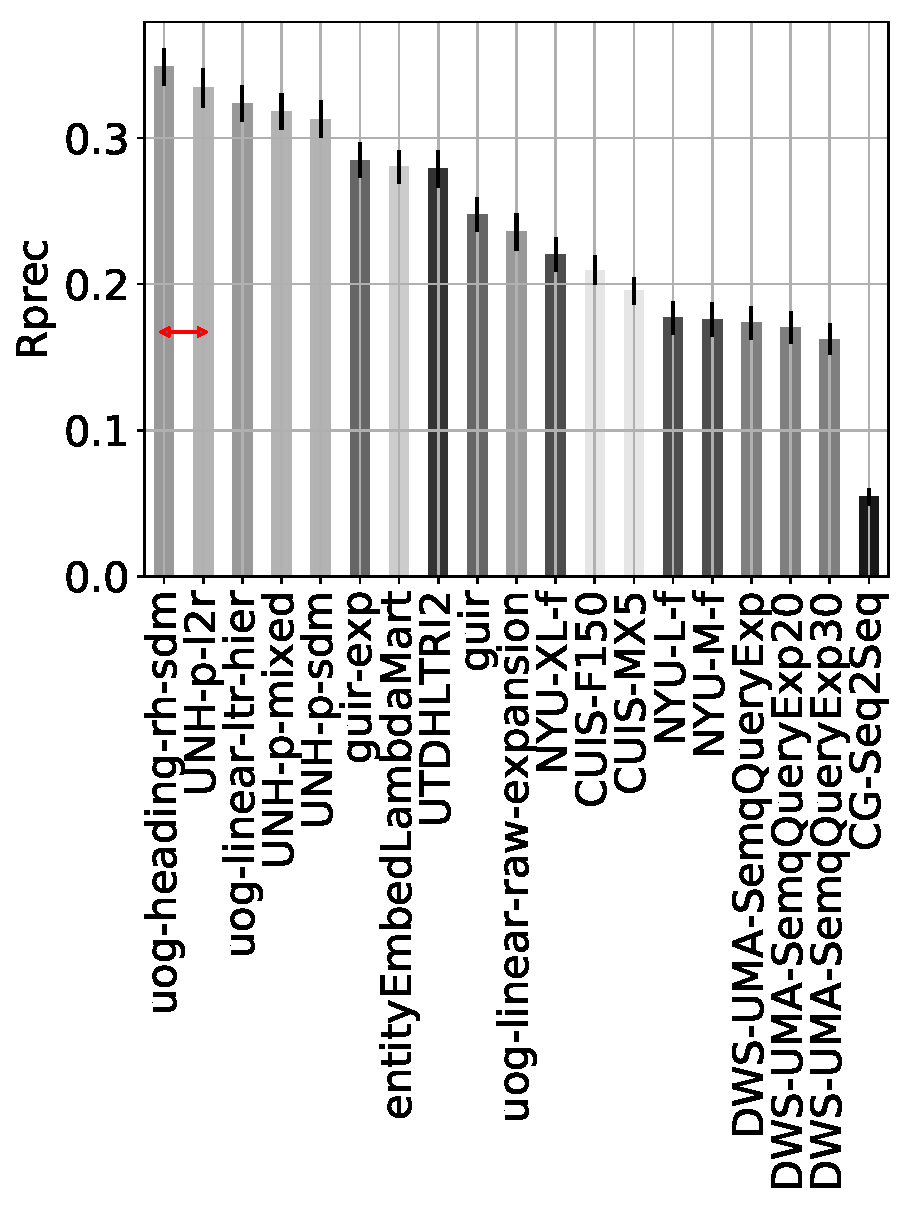
\includegraphics[width=0.45\columnwidth]{manual-psg-Rprec.pdf}}
    \hfill
    \subfloat[Entity Task]{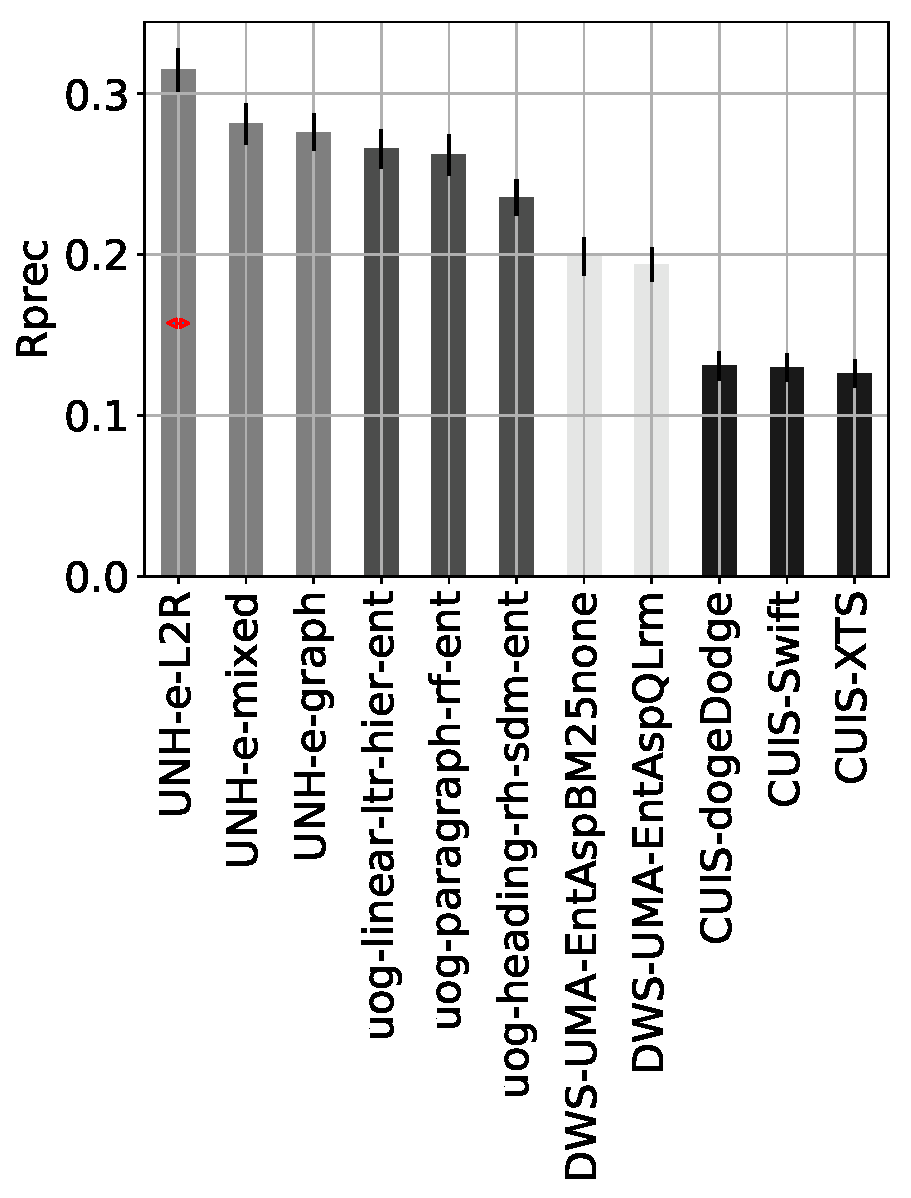
\includegraphics[width=0.45\columnwidth]{manual-entity-Rprec.pdf}}
    \caption{TREC CAR 2018 results for all participated systems, using the manual benchmark and Rprec as evaluation measure.}
    \label{fig:trec_2018_results}
\end{figure}

\begin{table}
\centering
\caption{Performance of entity retrieval methods. Y1 Train and Y2 Test benchmarks are derived from an automatically generated ground truth. The Y2 Test benchmark contains the TREC 2018 manual assessments.\label{tab:entity-results}}
\resizebox{\columnwidth}{!}{%
    \begin{tabular}{llllllllll}\toprule 
        \textbf{Method} & \multicolumn{3}{c}{\textbf{Y1 Train}} & \multicolumn{3}{c}{\textbf{Y1 Test}} & \multicolumn{3}{c}{\textbf{Y2 Test}} \\
        \cmidrule(lr){2-4} \cmidrule(lr){5-7} \cmidrule(lr){8-10}
        & \textbf{MAP} & \textbf{RPREC} & \textbf{NDCG} & \textbf{MAP} & \textbf{RPREC} & \textbf{NDCG} & \textbf{MAP} & \textbf{RPREC} & \textbf{NDCG} \\
        %\midrule
        UNH-e-l2r   & 0.15 & \textbf{0.17} & \textbf{0.42} & \textbf{0.17} & \textbf{0.18} & \textbf{0.44} & \textbf{0.31} & \textbf{0.31} & \textbf{0.51} \\
        UNH-e-graph & 0.14 & 0.15  & 0.34 & 0.14 & 0.16 & 0.34 & 0.27 & 0.28 & 0.48 \\
        UNH-e-sdm & 0.16 & 0.17  & 0.38 & 0.17 & 0.18 & 0.40 & 0.26 & 0.28 & 0.46 \\
        UNH-e-mixed & \textbf{0.16} & \textbf{0.17}  & 0.38 & \textbf{0.17} & \textbf{0.18} & 0.40 & 0.27 & 0.28 & 0.44 \\
         bm25-ecm & 0.11 & 0.12  & 0.32 & 0.10 & 0.12 & 0.32 & 0.18 & 0.19 & 0.42 \\
         ql-ecm & 0.11 & 0.13  & 0.33 & 0.11 & 0.13 & 0.32 & 0.17 & 0.19 & 0.40 \\
        \bottomrule
    \end{tabular}
    }
\label{tab:entity}
\end{table}


\begin{table}
\centering
\caption{Performance of passage retrieval methods (submitted and low-level sectionpath baselines). Y1 Train and Y1 Test benchmarks are derived from an automatically generated ground truth. The Y2 Test benchmark contains the TREC 2018 manual assessments.\label{tab:psg-results} }
\resizebox{\columnwidth}{!}{%
    \begin{tabular}{llllllllll}\toprule 
        \textbf{Method}  & \multicolumn{3}{c}{\textbf{Y1 Train}} & \multicolumn{3}{c}{\textbf{Y1 Test}} & \multicolumn{3}{c}{\textbf{Y2 Test}} \\
        \cmidrule(lr){2-4} \cmidrule(lr){5-7} \cmidrule(lr){8-10}
        & \textbf{MAP} & \textbf{RPREC} & \textbf{NDCG} & \textbf{MAP} & \textbf{RPREC} & \textbf{NDCG} & \textbf{MAP} & \textbf{RPREC} & \textbf{NDCG} \\
        %\midrule
        UNH-p-l2r             & 0.12                 & 0.09                  & 0.20                  & 0.13                & 0.11                  & \textbf{0.27}               & \textbf{0.34}                & \textbf{0.33}                  & \textbf{0.58}               \\ 
        UNH-p-SDM             & 0.15                 & 0.12                   & 0.25                  & 0.14                & \textbf{0.13}                  & 0.24               & 0.30                & 0.31                  & 0.47               \\ 
        UNH-p-mixed           & \textbf{0.16}                 & \textbf{0.14}                   & \textbf{0.25}                  & \textbf{0.15}                & \textbf{0.13}                  & 0.25               & 0.29                & 0.32                  & 0.47               \\ 
        bm25-none & 0.14                 & 0.11                   & 0.26                  & 0.13                & 0.10                  & 0.25               & 0.30                     & 0.30                       & 0.54                      \\ 
        ql-none   & 0.13                 & 0.10                   & 0.25                  & 0.13                & 0.10                  & 0.25               & 0.31                     & 0.32                       & 0.55                      \\ 
        ql-rm     & 0.08                 & 0.05                  & 0.24                  & 0.08               & 0.06                 & 0.20               & 0.23                    & 0.24                       & 0.47                      \\ 
        bm25-rm   & 0.11                 & 0.08                  & 0.24                  & 0.11                & 0.09                 & 0.24               & 0.29                     & 0.29                       & 0.52                      \\ \bottomrule
    \end{tabular}
    }
\label{tab:passage}
\end{table}


\FloatBarrier


% \begin{figure}%
%     \centering
%     \subfloat[label 1]{{\includegraphics[width=5cm]{img1} }}%
%     \qquad
%     \subfloat[label 2]{{\includegraphics[width=5cm]{img2} }}%
%     \caption{2 Figures side by side}%
%     \label{fig:example}%
% \end{figure}

\section{Evaluation on TREC News}


\begin{table}
\centering \caption{Performance of entity re-ranking methods on NEWS. $^{\triangledown}$marks
methods with significant difference to best performing method according
to a paired-t-test with $\alpha=0.05$.\label{tab:news-results}}
%\resizebox{\columnwidth}{!}{%
\begin{tabular}{llll}
\toprule 
\textbf{Method}  & \multicolumn{3}{c}{\textbf{NEWS}}\tabularnewline
\cmidrule(lr){2-4}  & \textbf{MAP}  & \textbf{RPREC}  & \textbf{NDCG@5} \tabularnewline
%\midrule 
UNH-ParaBm25 & $0.82\pm0.03$ & $0.72\pm0.04$ & $0.74\pm0.03$\tabularnewline
UNH-TitleBm25 & $0.81\pm0.03$ & $0.71\pm0.04$ & $0.72\pm0.03$\tabularnewline
UNH-ParaBm25Ecm & $0.71\pm0.04^{\triangledown}$ & $0.63\pm0.05^{\triangledown}$ & $0.55\pm0.04{}^{\triangledown}$\tabularnewline
%\midrule
\cmidrule(lr){2-4} 
median run & N/A & $0.66$ & $0.62$\tabularnewline
best run & N/A & $0.76$ & $0.82$\tabularnewline
\bottomrule
\end{tabular}

%} 
\end{table}

We participate in the NEWS track entity ranking task. As no training data was provided, we participate with with three variations of our low-level entity retrieval features as described in Section \ref{sec:entity}.

In this task, we are given a set of entities that we have to re-rank by importance for the article. Our approach is to use a part of the given news article (title or first paragraph) to construct a query. This query is used to retrieve entities from the entity index built from pages made available in CAR's allButBenchmark collection. We use BM25 with a whitelist to retrieve a re-ranking Wiki pages and rank the set of given entities according to their pages.

\begin{itemize}
    \item UNH-TitleBm25: Using the article title as a query, use BM25 to retrieve from the page index.  
    \item UNH-ParaBM25: Using the first paragraph (or at least 200 characters) of the news article's content as a query,  use BM25 to retrieve from the page index.  
    \item UNH-ParaBM25Ecm:  Using the first paragraph of the news article as query to retrieve CAR paragraphs. The ecm entitt ranking is derived from these paragraphs (using entity links provided by CAR organizers).
\end{itemize}

% The last method uses the entity context model in a non-standard way, where the whole page is used instead of short passages: After retrieving a feedback run of Wikipedia pages with BM25, each page is represented as bag-of-entity-link-targets. Using the relevance model \cite{lavrenko2017relevance}, we compute the distribution over expansion entities $P(E|Q)$. Instead of expanding the query with these entities, we use the distribution directly to produce a ranking of entities.
% 
% $$ score(E|Q)= \sum_{D\in \text{ranking}} p(D|Q) p(E|D)$$

The results are presented in Table \ref{tab:news-results}. We see that retrieving entities with the first paragraph (no ecm expansion) works best. For reference we include median and best run as provided by the NEWS organizers. Our best run performs above the median and slightly below the best run.


% Preview source code for paragraph 0
% Preview source code for paragraph 0





%In this notebook we experiment with methods of document retrieval that utilize the context of entity links for passage and entity retrieval. In the case of entity retrieval, we use the context in which an entity occurs in a passage as a means of indicating the relevance of an entity with respect to a query.
%This results in a significant improvement over just using features that score the relevance of an entity using fielded queries (such as the title, inlinks, or outlinks fields associated with a Wikipedia entity).
% We show that under the right conditions (e.g. with English stemmer) a combination of traditional retrieval methods results in best performance.


\section{Conclusion}
In this notebook we experiment with methods of document retrieval that  utilize the context of entity links for passage and entity retrieval.

In the case of CAR entity retrieval, we use the context in which an entity occurs in a passage as a means of indicating the relevance of an entity with respect to a query.
This results in a significant improvement over just using features that score the relevance of an entity using fielded queries (such as the title, inlinks, or outlinks fields associated with a Wikipedia entity).


While we were unable to show a similar improvement by retrieving passages using information pertaining to the entities it contains, we conclude that part of the reason for this not working was because entities are less ``specific' indicators of relevance than passages.
For example, while the entity ``United States'' may be relevant to a query, this does not necessarily indicate that all passages that contain the entity ``United States'' are relevant.
This suggests potential future work in understanding which entities are most important (salient) in indicating the relevance of passages that contain them.
 We show that under the right conditions (e.g., Lucene with English stemmer) a combination of traditional retrieval methods with learning to rank results in best performance.
 
On the NEWS entity ranking task we only retrieved entities from a Wikipedia dump, as no training data was provided. We see that using the first paragraph of the news article is as good as its title. 


 
In comparison to other participating teams in CAR and NEWS track, our methods placed either best or second-best.


% We present in this notebook methods which take advantage of semi-structured data from multiple sources (entities and passages) to improve retrieval results. We show that this approach is very effective in retrieving entities under the Entity Context Model.
% This notebook presents the methods of the team TREMA-UNH to TREC CAR and TREC News. 



\bibliographystyle{unsrt}
\bibliography{sample.bib}

\end{document}
